\section{Feature: Vaadin-Akka Integration}
\label{sec:feature-vaadin-akka}

The architecture on Section~\ref{sec:akkaria} describes a system with
\akka actors integrated in a \vaadin web application.
%
Today's story shows a possible implementation of such integration.  
\begin{feature}
  Vaadin-Akka Integration consists in the integration of a \vaadin web
  application with an \akka actor system to provide a highly scalable
  and performant web application. The integration architecture is
  shown in Figure~\ref{fig:vaadin-akka-integration}.
%




\begin{figure}[h]
  \centering
  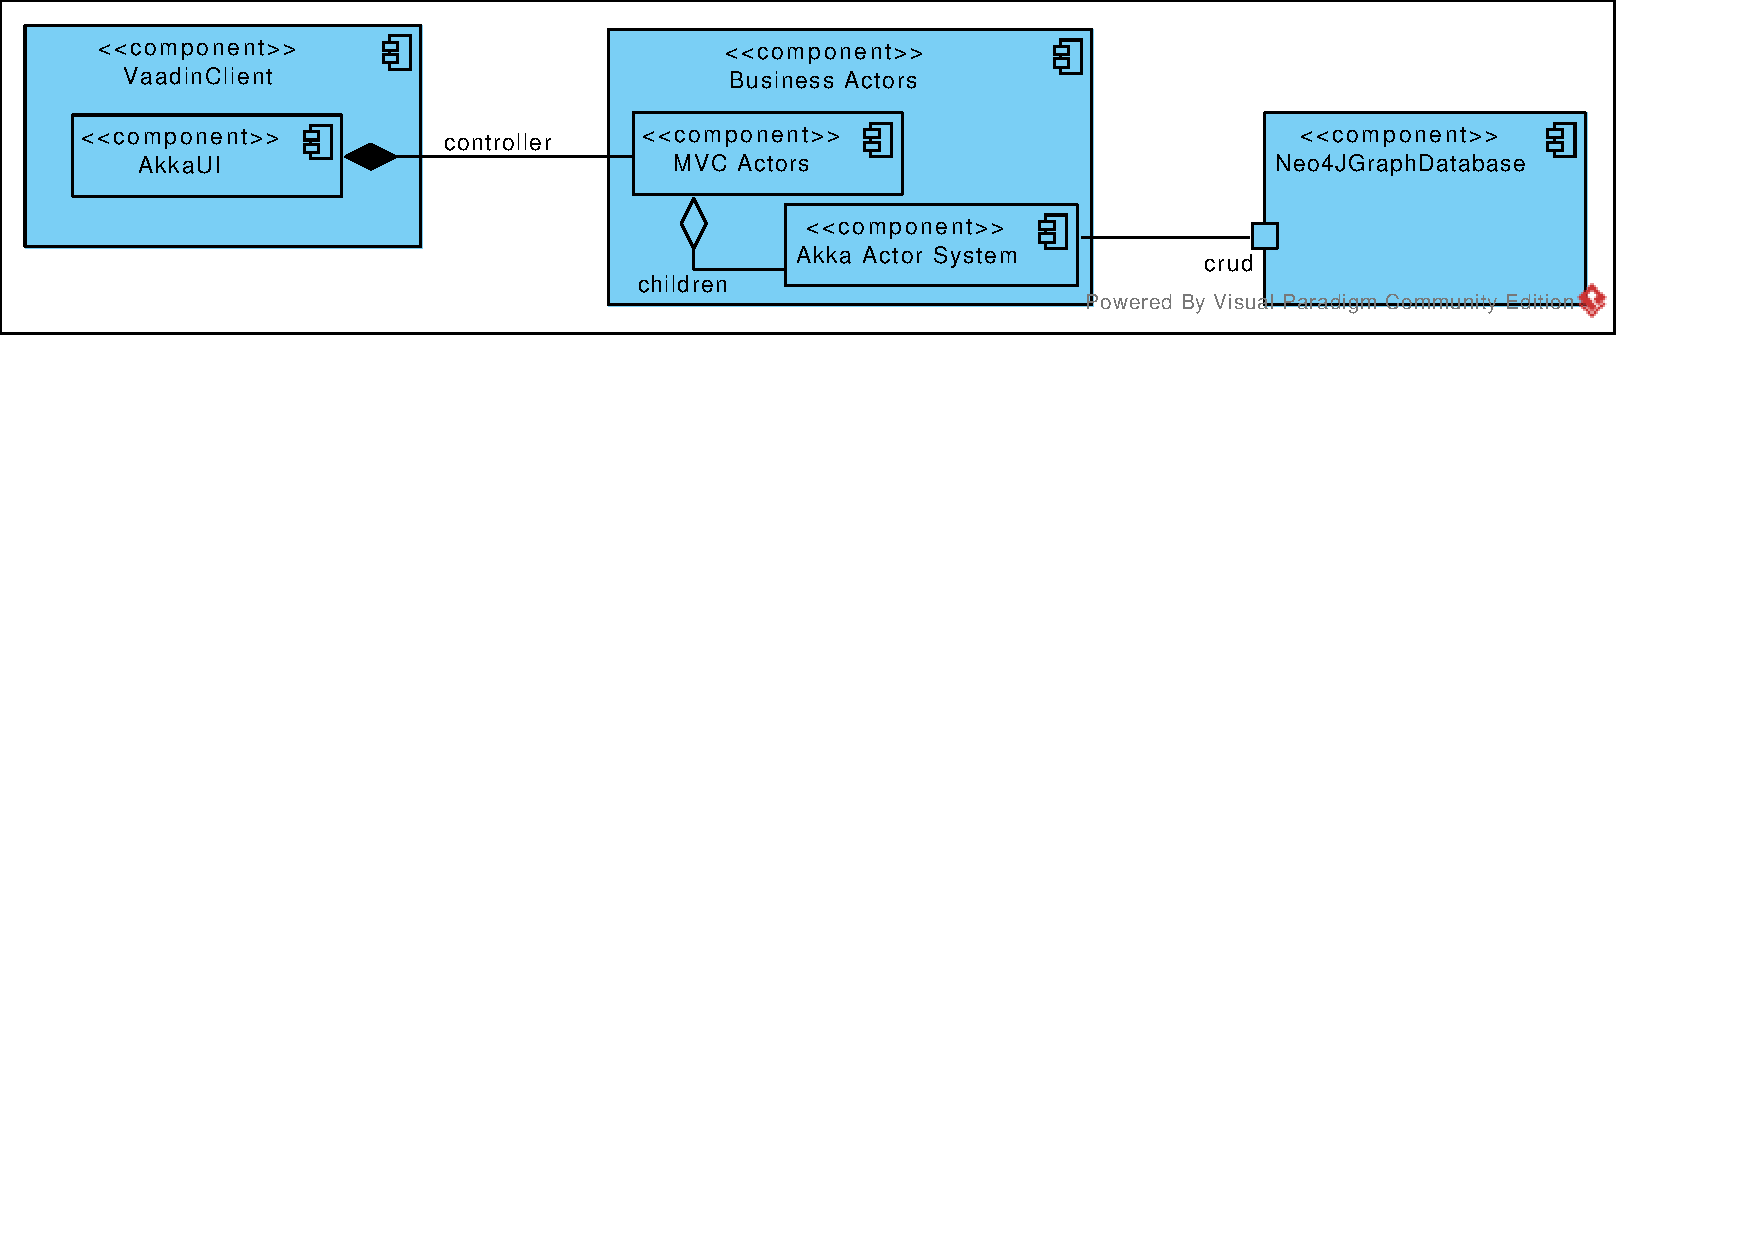
\includegraphics[scale=.45]{figures/VaadinAkkaIntegration.pdf}
  \caption{\vaadin-\akka integration. \vaadin subsystem provides a
    view for clients and communicates with the backend asynchronously
    via the \akka actor system}
  \label{fig:vaadin-akka-integration}
\end{figure}




%%% Local Variables:
%%% mode: latex
%%% TeX-master: "main"
%%% End:

%
  \begin{task}
    Create abstract class AkkaUI\\
    % \feature{feature/userUI/akkaUI}{done}
  \end{task}
  \begin{task}
    Rename MyUI to WelcomeUI\\
    % \feature{feature/userUI/akkaUI}{done}
  \end{task}
  \begin{task}
    Make WelcomeUI extend AkkaUI\\
    % \feature{feature/userUI/akkaUI}{done}
  \end{task}
  \begin{task}
    Create class UserUI extends AkkaUI\\
    % \feature{feature/userUI/akkaUI}{done}
  \end{task}
  \begin{task}
    Merge akkaUI with userUI\\
    % \feature{feature/userUI/akkaUI}{todo}
  \end{task}
%

  \begin{task}
    Determine the communication protocol in form of a session type
    specification\\
    % \feature{feature/task/specification}{todo}
  \end{task}
  \begin{task}
    Determine the client-side projection of the communication
    protocol\\
    % \feature{feature/task/specification/client}{todo}
  \end{task}
  \begin{task}
    Determine the server-side projection of the communication
    protocol\\
    % \feature{feature/task/specification/server}{todo}
  \end{task}
%

  \begin{task}
    Create tests that asserts about the behaviour expected by the
    specification, both on client and server sides. This tests should
    verify that:
    \begin{itemize}
    \item All expected messages are received\\
      \feature{feature/task/test/}{todo}
    \item All messages are processed in the order predefined by the
      session type
    \item If termination is mandatory, assert about termination status
    \end{itemize}
  \end{task}



\begin{task}
  Create WelcomeMVCActor, a subclass of MVCActor, as a
  static\footnote{Why \code{static}} inner class of WelcomeUI. This
  actor will implement the MVC pattern of this architecture:
  \begin{task}
    Implement the communication protocol inside the
    \code{onReceive()}, as asynchronously as possible.\footnote{Use
      \code{tell} and \code{forward} actor communication patterns and
      reserve the \code{ask} communication pattern for special cases.}
  \end{task}
  \begin{task}
    Use a \emph{session type based finite state machine} to guide
    communication dealing with message processing order.
  \end{task}
  \begin{task}
    Store incoming messages locally to decide how to proceed and react
    to them when; messages make the fsm to advance in the session type
    performing a state transition
  \end{task}
  \begin{task}
    Define server-side business actors as BusinessActors
  \end{task}
  \begin{task}
    Implement the server-side projection of the asynchronous
    communication protocol in the \code{onReceive()} method.
  \end{task}
\end{task}
%


\end{feature}




%%% Local Variables:
%%% mode: latex
%%% TeX-master: "main"
%%% End:
